\iffalse
\let\negmedspace\undefined
\let\negthickspace\undefined
\documentclass[journal,12pt,twocolumn]{IEEEtran}
\usepackage{cite}
\usepackage{amsmath,amssymb,amsfonts,amsthm}
\usepackage{algorithmic}
\usepackage{graphicx}
\usepackage{textcomp}
\usepackage{xcolor}
\usepackage{txfonts}
\usepackage{listings}
\usepackage{enumitem}
\usepackage{mathtools}
\usepackage{gensymb}
\usepackage{comment}
\usepackage[breaklinks=true]{hyperref}
\usepackage{tkz-euclide} 
\usepackage{listings}
\usepackage{gvv}                                        
\def\inputGnumericTable{}                                 
\usepackage[latin1]{inputenc}                                
\usepackage{color}                                            
\usepackage{array}                                            
\usepackage{longtable}                              
\usepackage{calc}                                             
\usepackage{multirow}                                         
\usepackage{hhline}                                           
\usepackage{ifthen}                                           
\usepackage{lscape}

\newtheorem{theorem}{Theorem}[section]
\newtheorem{problem}{Problem}
\newtheorem{proposition}{Proposition}[section]
\newtheorem{lemma}{Lemma}[section]
\newtheorem{corollary}[theorem]{Corollary}
\newtheorem{example}{Example}[section]
\newtheorem{definition}[problem]{Definition}
\newcommand{\BEQA}{\begin{eqnarray}}
\newcommand{\EEQA}{\end{eqnarray}}
\newcommand{\define}{\stackrel{\triangle}{=}}
\theoremstyle{remark}
\newtheorem{rem}{Remark}
\begin{document}

\bibliographystyle{IEEEtran}
\vspace{3cm}

\title{NCERT DISCRETE}
\author{EE23BTECH11020 - Raghava Ganji$^{*}$% <-this % stops a space 
}
\maketitle
\newpage
\bigskip

\renewcommand{\thefigure}{\theenumi}
\renewcommand{\thetable}{\theenumi}

\textbf{Question 10.5.3.5:}
The first term of an AP is $5$, the last term is $45$ and the sum is $400$. Find the number of terms and the common difference.\\
\textbf{solution:}\\
\fi
Given AP is 5, \ldots, 45.\\\\
\begin{table}[h]
\centering
\begin{tabular}{|c|c|c|}\hline
$x\brak 0$ & $5$ & 1st\hspace{1mm}term\\ \hline
$x\brak n$ & $45$ & \brak {n+1}th\hspace{1mm}term\\ \hline
$y\brak n$ & $400$ & sum\hspace{1mm}of\hspace{1mm}\brak {n+1}\hspace{1mm}terms\\ \hline
n+1 & ? & no.of\hspace{1mm}terms\\ \hline
d & ? & common\hspace{1mm}difference\\ \hline
\end{tabular}
\caption{parameters}
\end{table}

\begin{align}
x\brak n&=x\brak 0+nd\\
40&=nd\label{10.5.3.5.2}\\
y\brak n&=\frac{n+1}{2} \sbrak {2x\brak 0+nd}\\
\implies n&=15\label{10.5.3.5.4}\\
\implies d&=\frac{8}{3}\label{10.5.3.5.5}
\end{align}
by substituting equation \eqref{10.5.3.5.4} in the  equation \eqref{10.5.3.5.2}, we get the equation \eqref{10.5.3.5.5}.\\
z transform of $x\brak n,y\brak n$ are $X\brak z,Y\brak z$
\begin{align}
X\brak z&=\frac{7}{3\brak{1-z^{-1}}}+\frac{8}{3\brak{1-z^{-1}}^2}\\
Y\brak z&=\frac{7}{3\brak{1-z^{-1}}^2}+\frac{8}{3\brak{1-z^{-1}}^3}
\end{align}
\begin{figure}
    \centering
    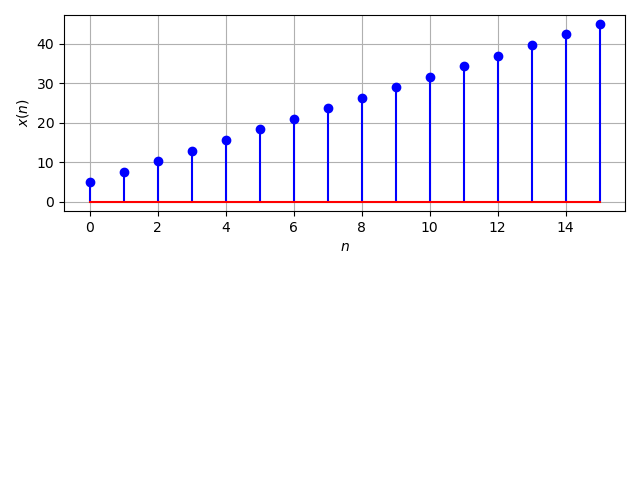
\includegraphics[width=1\columnwidth]{ncert-maths/10/5/3/5/figs/10.5.3.5.1.png}
    \caption{analysis of x\brak n}
\end{figure}
\begin{figure}
    \centering
    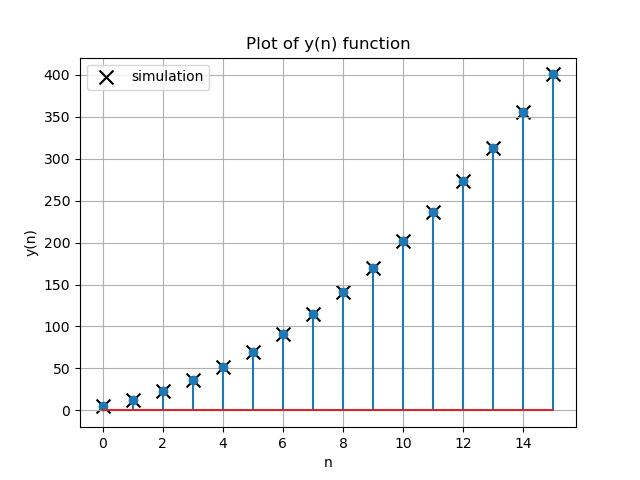
\includegraphics[width=1\columnwidth]{ncert-maths/10/5/3/5/figs/10.5.3.5.2.jpg}
    \caption{simulation vs analysis of y\brak n}
\end{figure}
%\end{document}
